\section{Exploring Interleaving Space}
\label{s:design}

\newcommand{\coverage}{XXX coverage\xspace}

\newcommand{\segment}{segment graph\xspace}
\newcommand{\segments}{segment graphs\xspace}
\newcommand{\Segments}{Segment graphs\xspace}

\begin{itemize}
\item our approach in one sentence: defining the universal set $U$
  using a coverage metric, and directing execution to consume the
  universal set
\item approach overview
  \item input: concurrent jobs and initial interleaving
  \begin{itemize}
    \item what are we going to do
      \begin{itemize}
      \item coverage
      \item interleaving mutation
      \end{itemize}
    \end{itemize}
\item coverage
  \begin{itemize}
  \item rationale:
  \item challenges:
  \item solution:
  \end{itemize}
  \item interleaving mutation
    \begin{itemize}
    \item rationale:
    \item challenges:
    \item solution:
    \end{itemize}
\end{itemize}


In this section, we describe our approach to explore the interleaving
space.
%
Our approach assumes that concurrent jobs (\eg, syscalls) and an
initial interleaving (= seed interleaving) of the concurrent job are
given as an input.
%
With the given input, our approach \textit{mutates the interleaving}
to produce other interleavings for exploring the interleaving space.

The key improvement of our approach is in adopting a novel coverage
metric to track multiple pairs of conflicting accesses (\eg,
$(\texttt{A1} \rightarrow \texttt{B1}) \wedge (\texttt{B4} \rightarrow
\texttt{A2})$ in \autoref{fig:cve-2019-6974}).
%
In particular, after collecting coverages from the given interleaving
using the coverage metric, we \textit{estimates the universal coverage
  set $U$}, a set of coverages that the given concurrent jobs possibly
execute.
%
And then, to produce other interleavings, our interleaving mutation is
\textit{directed towards undisclosed coverages in $U$} until $U$ is
exhausted.

In the following paragraphs, \autoref{ss:overview} first provides the
overview of our approach. Then, \autoref{ss:coverage} describes our
coverage metric in the concurrency dimension. Lastly,
\autoref{ss:scheduler} illustrates the interleaving mutation algorithm
that quickly saturates the coverage.



\subsection{Key Idea}
\label{ss:keyidea}

\cut{
\PP{Challenges}
%
Even though testing combinations of multiple conflicting accesses
provides a good bug-finding capability, one could argue that it may
require too many execution as the number of such combination is too
large.
}

\dr{wip.}

\begin{itemize}
\item what do we do to explore the interleaving space?
  \begin{itemize}
  \item We take an interleaving (= a totally ordered instruction sequence as an input)
  \item mutate an interleaving to generate another interleaving
  \item how?
    \begin{itemize}
    \item collect {C1, C2, ...} from the interleaving
    \item infer $U$, the universal set of coverage
    \item consume $U$ until it is empty
    \end{itemize}
  \end{itemize}
\item an intuition for a coverage
  \begin{itemize}
    \item observations
      \begin{itemize}
      \item interleavings are directed acyclic graph
      \item multiple pairs of conflicting accesses are a subgraph of an interleaving
      \end{itemize}
  \item we represent a coverage using a graph (?)
  \end{itemize}

\item an intuition for an interleaving mutation
  \begin{itemize}
  \item two observatrions
    \begin{itemize}
      \item many coverages can be executed together
      \item we can infer what coverages should be further tested
      \end{itemize}
  \item step 1: collect coverage
  \item step 2: inference of coverages to test
  \item step 3: collect coverages that can be tested together
  \item step 4: generate an interleaving to test
  \end{itemize}
\end{itemize}


Our intuition comes from an observation that even a non-failing
interleaving bears hints on which interleavings require further
testing.
%
For example, if two consecutive load operations reading from a memory
location are followed by a store operation writing to the same
location, we can easily deduce that there might be a single-variable
atomicity violation.
%
If we run an interleaving generated by rearranging these operations,
we can identify whether the atomicity violation actually occurs or
not.
%
Our approach to explore the interleaving space realizes this
intuition.


\begin{figure*}[t]
  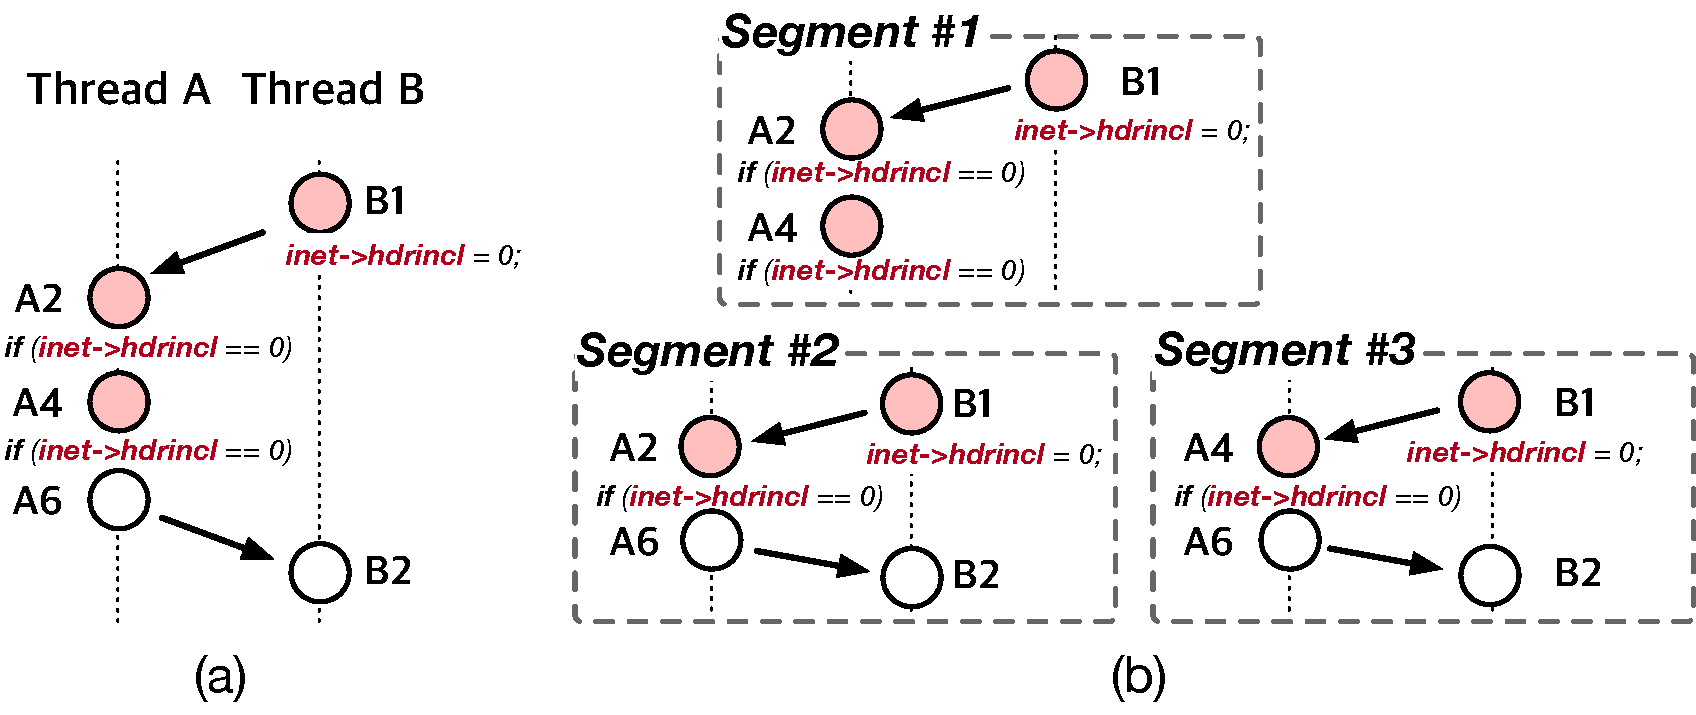
\includegraphics[width=0.9\linewidth]{fig/intuition.pdf}
  \caption{Key idea to explore the interleaving space. Each circle
    represents a memory access intruction. Annotations $R_x$ and $W_x$
    mean that the instruction reads from or writes to a memory
    location $x$ respectively.}
  \label{fig:intuition}
\end{figure*}


\PP{Overall steps}
%
Let us assume we obtain a totally ordered instruction sequence after
executing concurrent jobs~(\autoref{fig:intuition}-(a)).
%
In this instruction sequence, our purposes are 1) to track an
interesting behavior of the sequence, and 2) to schedule instructions
in the sequence for exposing more interesting behaviors.


As to tracking interesting behaviors, we follow the survey mentioned
in \autoref{ss:motivation} describing that most race conditions
deterministically manifest depending on a specific partial order of at
most four memory accesses.
%
According to this survey, such partial orders are ``interesting''
behaviors as they have a strong correlation to manifestation of
concurrency bugs.
%
Therefore, our purpose in tracking interesting behaviors in the
concurrency dimension turns into identifying how such partial orders
are established in the given sequence.
%
To this end, we enumerate small groups of a few (\eg, four) memory
accesses brought in the given instruction
sequence~(\autoref{fig:intuition}-(b)).
%
As the execution order of memory accesses in each group are already
determined, each group explains a part of the interleaving, therefore,
we call each group a segment of interleaving, or shortly a segment.
%
During fuzzing, we keep tracking segments as the signal of new
interelavings of concurrent jobs.





After collecting segments of concurrent jobs, we need to run the
concurrent jobs with different interleaving to observe different
segments.
%
Instead of blindly scheduling instructions, we deduce what partial
orders need to be explored in advance.
%
In other words, we hypothesize imaginary segments derived from
collected segments for further testing~(\autoref{fig:intuition}-(c)).
%
For example, by rearranging instructions of \texttt{Segment 1}, we
derive an imaginary segment called \texttt{Segment 1'} that are not
yet observed.
%
These imaginary segments will be used as scheduling hints; our
instruction scheduling mechanism will enforce imaginary segments
during further fuzzing runs.
%
It is worth noting that segments may be identical since the execution
order of not-conflicting instructions does not affect the outcome.
%
In this example, \texttt{Segment 1'} and \texttt{Segment 1''} are
identical and we consider they are redundant.

As a last step, we generate a hypothetical interleaving containing
these imaginary segments and run the interleaving to observe an
outcome~(\autoref{fig:intuition}-(d)).
%
Among all imaginary segments, some of them can be enforced together,
while some cannot.  For example, \texttt{Segment 1'} and
\texttt{Segment 2'} may be enforced together as they do not make a
conflict on the execution order of instructions.
%
We call two imaginary segments are harmonious if they are able to be
enforced together.
%
As all imaginary segments are not harmonious to all others, we need to
run different interleavings multiple times. For each fuzzing run, we
repeat generating a hypothetical interleaving by gathering harmonious
segments until we consume all imaginary segments.

\PP{Interleaving in a graph form}
%
Our interleaving exploration mechanism requires a few operations on an
interleaving such as 1) rearranging instructions in a segment, 2)
gathering harmonious segments, and 3) generating a whole interleaving
carrying multiple segments.
%
We notice that if we consider an interleaving as a graph of partial
orders, all above operations become simple graph operations.

From a given interleaving, we draw a graph consisting of vertices
representing memory access operations and edges representing the
execution order of the operations that may change the outcome if
reversed.
%
\dr{explain more intuition:}
With this graph, the required operations are simplified as follows: 1)
rearranging instructions is done by changing the direction of edges,
2) we can determine segments are harmonious if there is no loop in a
graph, and 3) a topological sort on a grpah generates a whole
interleaving.


In the rest of this section, we define the graph form of an
interleaving, and then provide details of the interleaving mutation.


% Dealing with an instruction sequence in this perspective has the
% following advantages:
% %
% First, it reduces the complexity of the interleaving space from
% exponential to polynomial to the number of instructions.
% %
% It is well known that the number of possible interleaving
% exponentially grows to the length of an instruction
% sequence~\cite{sctbench}. The intractable number of possible
% interleavings has been known as the paramount challenge for finding
% race conditions.
% %
% However, if we restrict our focus on a small number (\eg, four) of
% instructions, testing possible orders of small segments becomes a
% tractable problem with a polynomial complexity.
% %
% Second, given a concurrent jobs, it is able to know whether the
% concurrent jobs are worth further testing.
% %
% Because of the nondeterministic nature of race conditions, some race
% conditions hardly manifests even after a long period of
% testing~\cite{exprace}.
% %
% Without a proper metric, a fuzzer is forced to choose to repeatedly
% test a single input that does not causes a race condition, or to throw
% away an input that actually causes race condition when a very specific
% condition is satisfied.
% %
% Lastly, we can infer which segments are tested and which are not.
% %
% As mentioned before, some race conditions hardly manifests. These race
% conditions requires a very small race window sized for a few assembly
% instructions~\cite{afpacket}, or a thread stalling for a long
% time~\cite{noninclusive1, noninclusive2}. Although the probability of
% hitting the condition of them is not zero, without directing an
% interleaving, a fuzzer likely wastes a computing power until the
% condition is met.
% %
% Knowing which segments are not tested can significantly help for these
% cases. With a help of a scheduling hint-drected scheduler, we can
% force execution to experience segments that are not yet tested.


\subsection{Approach Overview}
\label{ss:overview}

Let us assume we have an input that consists of concurrent jobs.
%
While all possible interleavings of the concurrent jobs grows
exponentially to the number of memory access operations,






\PP{Interleaving in a graph form}
%
Assuming memory access operations in an interleaving are totally
ordered, the interleaving can be transformed into a directed acyclic
graph where vertices represent memory access operations, and edges
connect two vertices \texttt{v1} and \texttt{v2} if the \texttt{v1}
and \texttt{v2} correspond to a pair of conflicting accesses or
\texttt{v1} and \texttt{v2} are executed in the same thread. Each edge
is directed from \texttt{v1} to \texttt{v2} if \texttt{v1} is executed
before \texttt{v2}.


\autoref{fig:intuition} shows a directed acyclic graph representing a
totally ordered memory access operations,
$\texttt{A1} \rightarrow \texttt{B1} \rightarrow \texttt{B2}
\rightarrow \texttt{B4} \rightarrow \texttt{A2}$, that causes a
NULL-dereference bug in \autoref{fig:cve-2019-6974}.
%
In this graph, an edge \texttt{A1} and \texttt{B1}

as \texttt{A1} and \texttt{B1} conflict on \texttt{alloc->vma},

and


\PP{Coverage-directed interleaving mutation}





\subsection{Interleaving Graph}
\label{ss:coverage}

\newcommand{\mutable}{mutable edge\xspace}
\newcommand{\mutables}{mutable edges\xspace}
\newcommand{\immutable}{immutable edge\xspace}
\newcommand{\immutables}{immutable edges\xspace}


\begin{figure}[t]
  \caption{interleaving graph}
  \label{fig:interleaving-graph}
\end{figure}

In order to represent a partial order of memory accesses, we propose a
form of directed acyclic graph (DAG) called interleaving graph.
%
An interleaving graph describes an interleaving of concurrent jobs,
and represents partial orders between instructions.
%
In an interleaving graph, vertices indicate memory access operations,
and edges represent partial orders between these operations.
%
If there is a path from a vertex from another vertex, then the
execution order of two operations is established.

We categorize edges into two types, called \immutables and \mutables.
%
A \immutable corresponds to a program order in which instructions
appear on a thread~\cite{frightening, lkmm}. As a program order is
defined between instructions executed by the same thread, all
\immutables connect instructions from the same thread.
%
On the other hand, a \mutable is responsible to connect conflicting
instructions that 1) are executed by different threads, 2) access the
same memory location, and 3) at least one of them is write.
%
Therefore, the execution order of instructions connected by a \mutable
may directly affect the behavior of a program.


\autoref{fig:interleaving-graph} shows an example of an interleaving
graph.
%
\dr{TODO:}


\dr{TODO: imprecise description}
%
In terms of interleaving, \immutables and \mutables have different
properties. Let us suppose we have two interleaving graphs derived
from different interleavings of the same concurrent jobs.
%
As \immutables represent program orders, direction of \immutables does
not differ in the two interleaving graphs.
%
Whereas, a direction of \mutables may be different in the two
interleaving graphs.
%
It is worth noting that an edge may appear in only one interleaving
graph regardless of its type. This is because the control flow may be
changed according to the change of the data flow.


\PP{Segment of interleaving graph as coverage}
%
Although all execution order of conflicting instructions (\ie,
\mutables) in an interleaving graph may affect an outcome, we
concentrate on a small number of instructions because a few
instructions are enough to cause most ``interesting'' behaviors, \ie,
race conditions.

\dr{divide?}
%
We thus divide the interleaving graph into a set of subgraphs called
interleaving segment graphs, short for \segments.
%
While the interleaving graph represents a whole interleaving, an
\segment is a subgraph of the given interleaving graph that contains
two \mutables and at most four vertices. In addition, vertices in a
\segment are connected by at least one \mutable.

We capture \segments as coverage of a given interleaving of concurrent
jobs.
%
If a new \segment is not found while continuing to run the concurrent
jobs with different interleavings, the concurrent jobs unlikely expose
a race condition. In other words, if we collect all \segments of
concurrent jobs, we can lower the priority of the concurrent jobs.
%
It is worth noting that we select four as the maximum number of
vertices in a \segment because not only it is enough for most race
conditions, but also \dr{}...

In order to identify \segments from execution, we need to know the
total order of memory accesses. Otherwise, we may miss the execution
order between instructions so cannot faithfully capture \segments.
%
Therefore, our scheduling mechanism serializes execution of concurrent
jobs during fuzzing. Details are described later in \autoref{s:impl}.


\subsection{Interleaving Mutation}
\label{ss:scheduler}

% Since concurrent jobs may reveal different behaviors depending on an
% interleaving, a concurrency fuzzer adopt additional mutation strategy
% called interleaving mutation.

Our interleaving mutation is designed in a different way from previous
studies.
%
Instead of randomly selecting scheduling points~\cite{krace, ski} or
changing the execution order of a few instructions~\cite{razzer,
  snowboard}, we draw a whole hypothetical interleaving directed
towards uncaptured \segments.
%
To this end, our interleaving mutation consists of three steps:
%
1) identifying uncaptured \segments, 2) selecting \textit{harmonious}
\segments, and 3) generating scheduling points to test the selected
\segments.

\PP{Identifying uncaptured segment graphs}
%
Given \segments derived from an interleaving, identifying uncaptured
\segments is the first step of interleaving mutation for generating
another interleaving.
%
For each \segment, we change directions of \mutables to infer
uncaptured \segments.
%
As each \segment contains two \mutables, at most four uncaptured
\segments are derived for one \segment.

\dr{TODO:}...






\PP{Selecting interleaving segments to direct}
%
Given all uncaptured \segments, it is unlikely that all \segments can
be tested at once.
%
Our approach is to find out a subset of \segments that are
\textit{harmonious}. \Segments are harmonious if they do not form a
cycle in an imaginary graph.


It may require heavy computation to identify the largest subset that
are all harmonious to each other.
%
Instead of finding the optimal solution, we choose to use a greedy
algorithm.
%
Especially, given uncaptured \segments extracted from an interleaving
graph, our interleaving mutation starts by selecting a random
\segment.
%
And then it iteratively selects a \segment while confirming that the
selected \segment is harmonious.
%
Determining a given \segment is harmonious is conducted by checking a
loop in an accumulated interleaving graph.

\dr{TODO: describe an algorithm to check a loop. }
Its time complexity is $O(V)$.


\PP{Generating scheduling points}
%
After selecting harmonious \segments, generating scheduling points can
be easily done by conducting a topological
sort~\cite{topologicalsort}.
%
Since an imaginary interleaving graph is acyclic, a topological sort
always returns a sequence of vertices (\ie, instructions) that does
not violate a program order.
%
It is well known that the time complexity of a topological sort is
$O(V+E)$. Considering that the graph is sparse, $E$ is a small value
so the time complexity can be asymptotically considered as $O(V)$.
%
In this sequence, scheduling points are just instructions that the
preemption should happen; \ie, the next instruction is executed by a
different thread.
%


\dr{TODO: what if scheduling points are missing}


%%% Local Variables:
%%% mode: latex
%%% TeX-master: "p"
%%% End:
